95. $\cfrac{(x-1)(y-3)(y-2x)}{x-2}=0\Leftrightarrow \begin{cases}\left[\begin{array}{l}x=1,\\ y=3,\\ y=2x.\end{array}
ight.\\ x
eq2.\end{cases}$
$$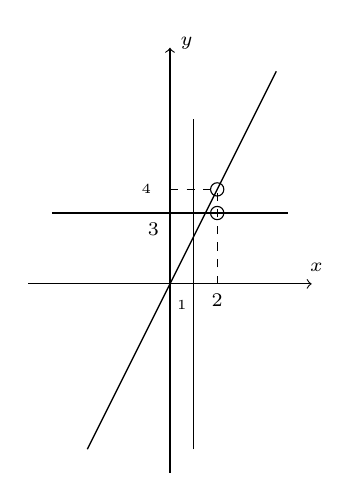
\begin{tikzpicture}[scale=0.3]
\tikzset {line01/.style={line width =0.5pt}}
\tikzset{line02/.style={line width =1pt}}
\tikzset{line03/.style={dashed,line width =0.5pt}}
%\filldraw [black] (0,0) circle (1pt);
\draw [->] (-6,0) -- (6,0);
\draw [->] (0,-8) -- (0,10);
\draw[line01] (-3.5,-7) -- (4.5,9);
\draw[line01] (1,-7) -- (1,7);
\draw[line01] (-5,3) -- (5,3);
\draw[line03] (2,0) -- (2,4);
\draw[line03] (0,4) -- (2,4);
%\draw[line03] (0,-2) -- (1,-2);
\draw (6.2,0.7) node {\scriptsize $x$};
%\draw (-1.2,-2) node {\scriptsize $-2$};
%\draw (-0.7,2) node {\scriptsize $2$};
%\draw (-0.7,1.2) node {\scriptsize $1$};
\draw (-1,4) node {\tiny $4$};
\draw (-0.7,2.3) node {\scriptsize $3$};
\draw (2,-0.7) node {\scriptsize $2$};
\draw (0.5,-0.9) node {\tiny $1$};
\draw (0.7,10.2) node {\scriptsize $y$};
\draw (2,4) circle (8pt);
\draw (2,3) circle (8pt);
%\draw (-2,-3) circle (8pt);
\end{tikzpicture}$$
